\documentclass[11pt]{article}
\usepackage[letterpaper, margin=0.8in]{geometry}
\usepackage{amsmath}
\usepackage{amssymb}
\usepackage{wrapfig}
\usepackage[makeroom]{cancel}
\usepackage{bbm}
\usepackage{booktabs}
\usepackage{float}
\usepackage{array}
\usepackage{bm}
\usepackage{enumerate}
\usepackage{amsfonts} 
\usepackage{color}
\usepackage{hyperref}
\usepackage{xcolor}
\usepackage{hyperref}
\usepackage{newfloat}
\usepackage{graphicx}
\usepackage{caption}
\usepackage{bbm}
\usepackage[overload]{empheq}
\newcommand{\IF}{\text{if }}
\def\changemargin#1#2{\list{}{\rightmargin#2\leftmargin#1}\item[]}
\let\endchangemargin=\endlist 
\newcommand{\norm}[1]{\left\lVert#1\right\rVert}

\begin{document}
\subsection*{Problem Set-up : Two Variance Components}
\subsubsection*{Two variance components}
The $p \times n$ data matrix $Y$ has measurements in $p$ probes for $n$ individuals. Then we use the following model:
\begin{equation}
Y_{ij} = \phi_i \Theta_{ij} + \epsilon_{ij}
\end{equation}
$\phi_i$ is the $i$'th probe effect where $\Theta_{ij}$ is a true count. $\epsilon_{ij}$ is an error term that follows a distribution of $\sim N(0, \delta_j^2 + \epsilon_i^2)$. Our objective is therefore to minimize the following:
\begin{equation}
\sum_{i=1}^{p} \sum_{j=1}^{n} \frac{(Y_{ij} - \phi_i \Theta_{ij})}{\sigma_i^2 + \delta_j^2} ^2 + \lambda \frac{\|\Theta_{i+1,\cdot} - \Theta_{i, \cdot}\|}{w_i}
\end{equation}



\subsection*{Alternating Descent}

We will build on the existing algorithm in that we add a conditional update of $\sigma$ and $\delta$ given $\phi$ and $\Theta$. Therefore, our three steps will be

\begin{itemize}
\item
Update $\sigma$ and $\delta$ given $\phi$ and $\Theta$ through likelihood maximization with gradient descent
\item
Update $\Theta$ given $\phi$, $\sigma$, $\delta$ through Group Fused Lars
\item
Update $\phi$ given $\Theta$, $\sigma$, $\delta$ by solving least squares

\end{itemize}


\subsection*{Estimating $\sigma$ and $\delta$ given $\Theta$ and $\phi$}

Assuming normality and mean 0 in the data $Y$, we can estimate $\sigma$ and $\delta$ through maximizing the likelihood. The log-likelihood of $Y$ is
\begin{equation}
\ell(Y; \sigma, \delta) = -\frac{np}{2}log(2\pi)
-\frac{1}{2} \sum_{i,j} log(\sigma_i^2 + \delta_j^2) - \sum_{i,j} \frac{Y_{ij}^2}{2(\sigma_i^2 + \delta_j^2)}
\end{equation}
\noindent and this leads to the gradient functions
\begin{align}
\frac{\partial \ell}{\partial \sigma_i} &= \sum_j 
\frac{ -\sigma_i^3 + \sigma_i (Y_{ij}^2 - \delta_j^2)}{(\sigma_i^2 + \delta_j^2)^2}\\
\frac{\partial \ell} {\partial \delta_j} &= \sum_i
\frac{-\delta_j^3 + \delta_j (Y_{ij}^2 - \sigma_i^2)}{(\sigma_i^2 + \delta_j^2)^2}
\end{align}

\noindent In order to make the above score functions to be zero, and assuming that $\sigma_i$ and $\delta_j$ are not 0 for all $i$ and $j$,

\begin{align}
\sum_{j=1}^{n} \frac{\sigma_i^2}{(\sigma_i^2 + \delta_j^2)^2} &= \sum_{j=1}^{n} \frac{Y_{ij}^2 - \delta_j^2}{(\sigma_i^2 + \delta_j^2)^2}\\
\sum_{i=1}^{p} \frac{\delta_j^2}{(\sigma_i^2 + \delta_j^2)^2} &= \sum_{i=1}^{p} \frac{Y_{ij}^2 - \sigma_i^2}{(\sigma_i^2 + \delta_j^2)^2}
\end{align}

\noindent Codes implementing gradient descent with line search based on the above are implemented in cnvJoint.


\subsection*{Estimating $\Theta$ given $\phi$, $\sigma$ and $\delta$}

In order to take advantage of the Group Fused Lars algorithm, we need to define the $(p-1) \times p$ change matrix $\Delta$ derived from the matrix $\Theta$ :
\begin{equation}
\Delta_{i \cdot} = \frac{\Theta_{i+1 \cdot}-\Theta_{i \cdot}}{w_i}
\end{equation}
\noindent and naturally
\begin{equation}
\Theta_{i\cdot} = \Theta_{1\cdot} + \sum_{s=0}^{i-1} w_s \Delta_{s \cdot}
\end{equation}
Our objective is then

\begin{equation}
Q_2(\phi, \Theta_{1\cdot}, \Delta) = 
\sum_{i=1}^{p} \sum_{j=1}^{n} \left(
\frac{
Y_{ij}-\phi_i \Theta_{1j} - \phi_i \sum_{x=0}^{i-1} w_s \Delta_{s\cdot}
}{
\sqrt{\sigma_i^2 + \delta_j^2}
}\right)^2 
 + \lambda \sum_{i=1}^{p-1} \| \Delta_{i \cdot} \| _2
\end{equation}
\noindent where $\Theta_{1\cdot}$ given $\Delta$ and $\phi$ is like below.
\begin{equation}
\Theta_{1\cdot} = \frac{
\sum_{i=1}^{p} \phi_i Y_{i\cdot} - \sum_{i=1}^{p} \phi_i^2 \sum_{s=0}^{i-1} w_s \Delta_s{\cdot}
}
{\sum_{i=1}^{p} \phi_i^2}
=
\frac{\phi^T Y - \phi^T T \Delta}{\phi^T \phi}
\end{equation}
\noindent where $T$ is known:
$$T=\begin{bmatrix}
0 & 0 & 0 & ... &0\\
\phi_2 w_1 & 0 & 0 & ... & 0\\
\phi_3  w_1 & \phi_3 w_2 & 0 & ... & 0\\
... & ... & ... & ... & ...\\
\phi_{p-1} w_1 & \phi_{p-1} w_2 & \phi_{p-1}w_3 & ... & 0\\
\phi_p w_1 & \phi_p w_2 & \phi_p w_3 & ... & \phi_p w_{p-1}
\end{bmatrix}
$$

\noindent So far, we only focused on removing $\Theta$ and write the objective with $\Delta$ in order to simplify the penalty term. Our final objective with no $\Theta$ term looks like this.

\begin{equation}
Q_3(\phi, \Delta, \sigma, \delta) = 
\sum_{i=1}^{p} \sum_{j=1}^{n}
\left(
\frac{
Y_{ij} - \phi_i 
\left(   \frac{\phi^TY_{\cdot j}}{\phi^T \phi} - \frac{\phi^T T \Delta_{\cdot j}}{\phi^T \phi}
  \right)
- \phi_i \sum_{s=0}^{i-1} w_s \Delta_{sj}
}
{
\sqrt{\sigma_i^2 + \delta_j^2}
}
\right)^2
 + \lambda \sum_{i=1}^{p-1} \| \Delta_{i\cdot}\|_2
\end{equation}

\noindent Above is equivalent to 
\begin{equation}
Q_3(\phi, \Delta, \sigma, \delta) = \sum_{i=1}^{p} \sum_{j=1}^{n} \frac{ \left((Q_{\phi}Y - Q_{\phi} T \Delta)_{i,j}\right)^2}{\sigma_i^2 + \delta_j^2} + \lambda \sum_{i=1}^{p-1} \|\Delta_{i \cdot}\|_2
\end{equation}
\noindent with $Q_{\phi} = I-(\phi^T\phi)^{-1} \phi \phi^T$.\\

\noindent Our goal is to modify the above objective $min_\Delta Q_3(\phi,\Delta,\sigma,\delta)$ to something like below with known $A$ and $B$.
\begin{equation}
min_\Delta  \| A - B \Delta\|_F^2 + \lambda \sum_{i=1}^{p} \| \Delta_{i, \cdot}\|
\end{equation}
Therefore, we need to transform $Q_{\phi}Y$ and $Q_{\phi}T$ in terms of $\sigma$ and $\delta$ so that, with $A(\phi, \sigma, \delta, w)$ and $B(\phi, \sigma, \delta, w)$,
\begin{equation}
\sum_{i=1}^{p} \sum_{j=1}^{n} \frac{ \left((Q_{\phi}Y - Q_{\phi} T \Delta)_{i,j}\right)^2}{\sigma_i^2 + \delta_j^2}
=
\|A-B\Delta\|_F^2
\end{equation}

\noindent Note the dimension of the matrices
\begin{align*}
Q_{\phi} &: p \times p\\
Y &: n \times p\\
T &: p \times (p-1)\\
\Delta &: (p-1) \times n
\end{align*}

\begin{itemize}
\item \textbf{get A}\\
Since $Y$ has dimension $p \times n$, we can do element-wise division of $Y$ to get $$\tilde{Y} = Y \odot \Lambda$$
where $\odot$ is Hadamard multiplication and $\Lambda$ is the $n \times p$ variance matrix so that $$\Lambda_{ij} = \sqrt{\frac{1}{\sigma_i^2 + \delta_j^2}}$$
Then, $$A = Q_{\phi} \tilde{Y}$$
\item \textbf{get B}\\
\noindent
Since we need to keep $\Delta$ intact, we will have to modify $Q_{\phi}T$ which is a $p \times (p-1)$ matrix. Since the variance component has the cell index $j$, we will need $n$ different versions of $Q_{\phi}T$ scaled differently for each $j$. This leads to a three-dimensional array $p \times (p-1) \times n$, and I don't think Group Fused Lars can handle this? :(




\end{itemize}
\subsection*{Data Simulation}
We assume the model (1) is true, and create data Y according to the model. The simulation follows the process below.

\begin{itemize}
\item
Fix the number of probes $p$ and the number of cells $n$ where $p > n$.
\item
Determine $\frac{n}{2}$ change points by taking a random sample from $1$ to $n$.
\item
Create $\Theta$. First divide $p$ probes into blocks according to the change points earlier determined. Then sample a random integer from $-10$ to $10$ for each block. All cells share the same $\Theta$. ($\Theta_{\cdot j} = \Theta_{\cdot k}$ for all $j, k = 1, .., n$)
\item
Create $\phi$ by sampling $p$ numbers from $N(0,1)$.
\item
Create cell-specific true variance $\delta_j^2$ from $unif(0.1, 1)$ for $j = 1, .., n$
\item
Create probe-specific true variance $\sigma_i^2$ from $unif(0.1, 1)$ for $i = 1, .., p$
\item
Sample $\epsilon_{ij} \sim N(0, \delta_j + \sigma_i)$
\item
Finally, make data Y by the formula $Y_{ij} = \phi_i \Theta_{ij} + \epsilon_{ij}$
\end{itemize}

\pagebreak

\subsection*{Problem set-up : Add cell-specific fixed effects}

\begin{equation}
Y_{ij} = \Theta_{ij} (\phi_i + \xi_j) + \epsilon_{ij}, \text{  } \epsilon_{ij} \sim N(0, \sigma^2)
\end{equation}

\begin{equation}
min_{\phi, \xi, \Theta} \text{ } \left(Y_{ij}-(\phi_i+\xi_j) \Theta_{ij} \right)^2 + \lambda \frac{\| \Theta_{i+1, \cdot} - \Theta_{i,\cdot}\|}{w_i}
\end{equation}

\subsection*{Alternating Descent}
\begin{itemize}

\item
Update $\Theta$ given ($\phi$ and $\xi_j$) through group fused lasso
\item
Update $\phi$ given ($\Theta$ and $\xi$) through solving least squares below where the left hand side is known
$$Y_{ij} - \Theta_{ij} \xi_j = \Theta_{ij} \phi_i  + \epsilon_{ij}$$
\item
Update $\xi$ given ($\Theta$ and $\phi$) through solving least squares
$$Y_{ij} - \Theta_{ij}\phi_i = \Theta_{ij} \xi_j + \epsilon_{ij}$$

\end{itemize}

\subsection*{Modify group fused lasso to accommodate $\xi$}
Define 
$$\Theta_{ij} = \Theta_{1j} + \sum_{s=0}^{i-1} w_s \Delta_{sj}$$
Then our problem becomes
\begin{align}
\min_\Theta \sum_{i,j} 
\left(
Y_{ij} - (\phi_i + \xi_j) \Theta_{1j} - (\phi_i + \xi_j) \sum_{s=0}^{i-1}w_s \Delta_{sj}
\right)^2
\end{align}
and our goal is to change this in the form of $\| A - B\Delta\|^2_F$. Given $\phi$, $\xi$, and $\Delta$, we can solve for $\theta_{1j}$ like below 

\begin{align*}
\Theta_{1j} &= \frac{
\sum_i (\phi_i + \xi_j) Y_{ij} - \sum_i (\phi_i + \xi)^2 \sum_{s=0}^{i-1} w_s \Delta_{sj}
}{\sum_i (\phi_i + \xi_j)^2}\\
&= \frac{
\phi^T Y_{\cdot j} + (\xi_j 1^T_p) Y_{\cdot j} - \phi^T T \Delta_{\cdot j}
- w\sum_i \phi_i \xi_j \sum_{s=0}^{i-1} w_s \Delta_{sj}
+ \sum_i \xi_j^2 \sum_{s=0}^{i-1} w_s \Delta_{sj}
}{\phi^T \phi + \phi^T (\xi_j 1_p) + \xi_j ^2}\\
\\
&\text{and this leads to the following vectorization }\\
\\
\Theta_{1 \cdot} & = \left(\phi^TY + 1_p^T Y \Xi - \phi^T T \Delta - 2(\phi^T W \Delta + 1_p^T W \Delta \Xi )  + 1_p^T W \Delta \Xi^2\right) \oslash \left( \phi^T \phi 1_n + (\phi^T 1_p)\xi + \Xi \xi\right)
\end{align*}

by introducing $W$ matrix and $\Xi$ matrix as following

\begin{align*}
W_{p \times (p-1)}& = \begin{bmatrix}
0 & 0 & 0 & ... &0 \\
w_1 & 0 & 0 & ... & 0\\
w_1 & w_2 & 0 & ... & 0\\
... & ... & ... & ... & ...\\
w_1 & w_2 & w_3 & ... & 0\\
w_1 & w_2 & w_3 & ... & w_{p-1}
\end{bmatrix}\\
\Xi_{n \times n} &= \begin{bmatrix}
\xi_1 & 0 & ... & 0\\
0 & \xi_2 & ... & 0\\
... & ... & ... & ...\\
0 & 0 & ... & \xi_n
\end{bmatrix}
\end{align*}

Also, the last part $(\phi_i+\xi_j) \sum_{s=0}^{i-1} w_s \Delta_{sj}$ can also be vectorized like the following.

$$
\phi_i \sum_{s=0}^{i-1} w_s \Delta_{s \cdot} + \sum_{s=0}^{i-1} w_s \Delta_{s\cdot} \Xi
$$

Lastly, note that the matrix $T$ is equal to $1\phi^TW$\\

Combining the above vectorizations, we can re-write the objective (18):
\begin{align*}
\sum_i \norm{ Y_{i\cdot} - \phi_i \left(  \frac{
\phi^T Y + 1_p^T Y \Xi - \phi^T 1\phi^TW \Delta - 2\phi^TW\Delta - 21_p^TW\Delta\Xi + 1_p^T W \Delta \Xi^2 }{\phi^T \phi 1_n + (\phi^T 1_p) \xi + \Xi \xi}    \right) - \phi_i \sum_{s=0}^{i-1} w_s \Delta_{s\cdot} (I_n+\Xi)
}^2
\end{align*}
\begin{align*}
= \sum_i \norm{
Y_{i\cdot} - \phi_i \left(
\frac{
\phi^T Y + 1_p^T Y\Xi + (-\phi^T1\phi^T - 2\phi^T) W\Delta - 1_p^TW\Delta(2\Xi - \Xi^2)
}{
\phi^T \phi 1_n + (\phi^T 1_p) \xi + \Xi \xi
}
\right)
-1\phi^TW\Delta (I_n+\Xi)
}^2
\end{align*}
where the fraction shows element-wise division. 

\pagebreak
\subsection*{Problem set-up : Add cell-specific perturbations}

\begin{equation}
Y_{ij} = (\Theta_{ij}+\xi_j)\phi_i + \epsilon_{ij}, \text{  } \epsilon_{ij} \sim N(0, \sigma^2)
\end{equation}

\begin{equation}
min_{\phi, \xi, \Theta} \sum_{i,j} (Y_{ij} - \xi_j \phi_i - \phi_i \Theta_{ij})^2 + \sum_{i}^p \lambda \frac{\|\Theta_{i+1\cdot} - \Theta_{i\cdot}  \|}{w_i}
\end{equation}


\subsection*{Alternating Descent}
\begin{itemize}

\item
Update $\Theta$ given ($\phi$ and $\xi$) through group fused lasso\\
This is exactly same as the original problem if we replace $Y_{ij}$ with $Y_{ij} - \phi_i\xi_j$ for each $i$ and $j$ with known $\phi_i$ and $\xi_j$.
\item
Update $\phi$  given ($\xi$ and $\Theta$) by solving least squares
$$\sum_{i,j}(Y_{ij} - (\Theta_{ij}+\xi_j)\phi_i)^2$$
$$\Rightarrow \phi_i = \frac{\sum_j (\Theta_{ij} + \xi_j)Y_{ij}}{
\sum_j (\Theta_{ij}+\xi_j)^2
}$$
\item
Update $\xi$ given ($\phi$ and $\Theta$) by solving least squares
$$\sum_{i,j} (Y_{ij} - \phi_i \Theta_{ij} - \phi_i \xi_j)^2$$
$$\Rightarrow \xi_j = \frac{
\sum_i (Y_{ij}-\phi_i \Theta_{ij})\phi_i
}{
\sum_i \phi_i^2
}$$

\end{itemize}

\subsection*{Constraints for identifiability}
We limit the L2 norm of $\phi$ to the length of the vector $\phi$, and we constrain the mean of $\xi$ to be 0. 

\subsection*{Performance Comparison}

Run the algorithm for
\begin{equation}
min_{\phi, \xi, \Theta} \sum_{i,j} (Y_{ij} - \xi_j \phi_i - \phi_i \Theta_{ij})^2 + \sum_{i}^p \lambda \frac{\|\Theta_{i+1\cdot} - \Theta_{i\cdot}  \|}{w_i}
\end{equation}
and 
\begin{equation}
min_{\phi, \Theta} \sum_{i,j} (Y_{ij} - \phi_i \Theta_{ij})^2 + \sum_{i}^p \lambda \frac{\|\Theta_{i+1\cdot} - \Theta_{i\cdot}  \|}{w_i}
\end{equation}
And label the estimates from each algorithm (1) and (2). We compare $\Theta^{(1)}$ and $\Theta^{(2)}$, and so on.

Now compare,
\begin{itemize}

\item
We look at $\xi_j^{(1)} \phi_i^{(1)} + \phi_i^{(1)}\Theta_{ij}^{(1)}$ and $\phi_i^{(2)}\Theta_{ij}^{(2)}$, and how close they are to $Y_{ij}$ for each $i$ and $j$ (equivalent to comparing RSS).

\item
We look at $\Theta^{(1)}$ and $\Theta^{(2)}$ only which in theory should represent the true copy number of each sample.

\item
We look at $\Theta^{(1)} + \xi$ and $\Theta^{(2)}$

\item
We look at the minimized value that includes the penalty term, or the optimized value of (21) and (22). 

\end{itemize}

\section{Results}
We ran the chromosome 22 data on both models, with and without $\xi$. For the reference, the points and lines labeled `after xi' is
$$Y_{ij} = (\Theta_{ij} + \xi_j)*\phi_i + \epsilon_{ij}$$
and those labeled `before xi' is
$$Y_{ij} = \Theta_{ij} * \phi_i + \epsilon_{ij}$$

In this section, we only focus on the first four samples and the last four samples (1, 2, 3, 4, 29, 30, 31, 32). This is designed to check the performance on the two distinct cell types. It is also appropriate in that top 5 samples with the largest $\xi$ in magnitude are 3, 27, 12, 23, and 30, and two of them (samples 3 and 30) are included in our panels. 


The first thing I checked was the AIC, BIC, and RSS error plots in Figure \ref{errorplots}. The red line is after implementing $\xi$. 

\begin{figure}[h]
\centering
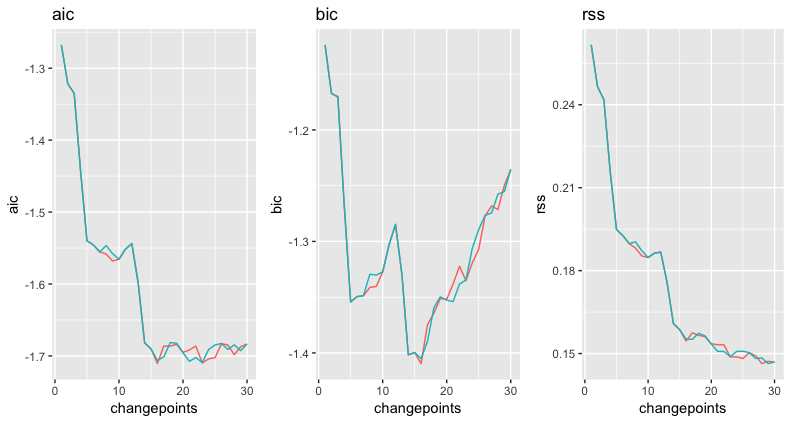
\includegraphics[width=0.7\textwidth]{errorplot.png}\\
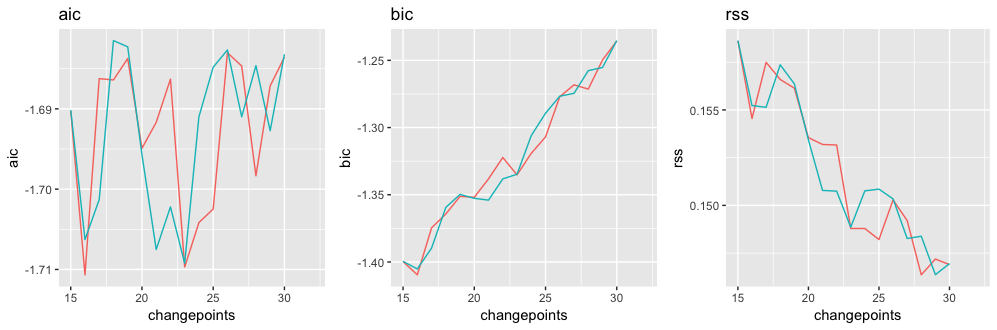
\includegraphics[width=0.7\textwidth]{errorplot2.png}
\caption{The error rates are mostly similar before and after the implementation if xi. Even when we zoom into the low-error region, it is difficult to decide which method performs better. Both the minimum of aic and bic error is achieved by the model with $xi$, but the error is so small that it seems possible that they're due to numercal instability.}
\label{errorplots}
\end{figure}

\pagebreak

Then, we checked $\Theta_{ij}\phi_i$. The primary goal is to check the alignment with zero. The original model without cell specific effects seem to perform better assuming that certain sections actually have true values of 0. See Figure \ref{thetaphi}.
\begin{figure}[h]
\centering
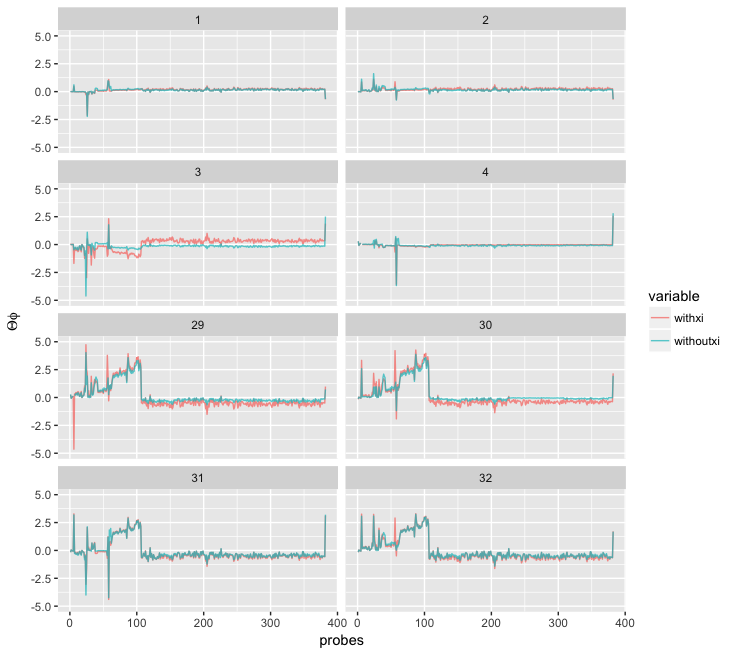
\includegraphics[width=0.6\textwidth]{thetaphi.png}
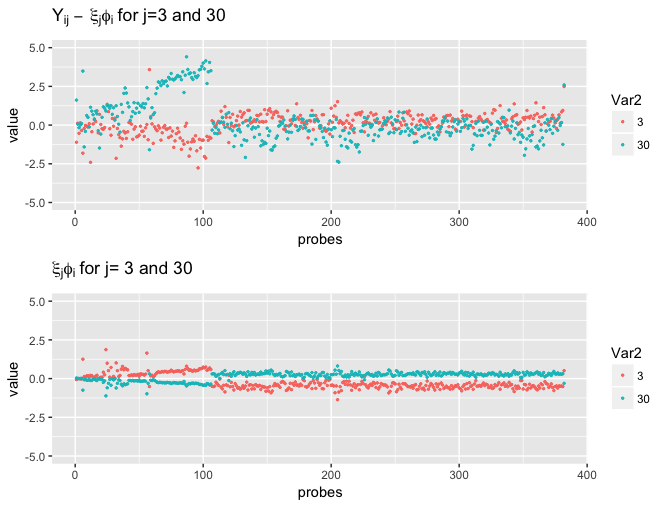
\includegraphics[width=0.5\textwidth]{zoomedin.png}
\caption{We assume the first four samples have zero over the entire chromosome. I also expect that for samples 29 to 32, probes from around 100 to the end have theta values zero. Some results are similar while samples 3, 29, and 30 show some difference. Overall, the model with $\xi$ shows more variability, especially for samples where $xi$ is large.}
\label{thetaphi}
\end{figure}


\pagebreak

Finally, we compare $\Theta$ only. $\Theta$ is supposed to represent the true values of the copy number, so it is important that it is aligned at 0. 

\begin{figure}[h]
\centering
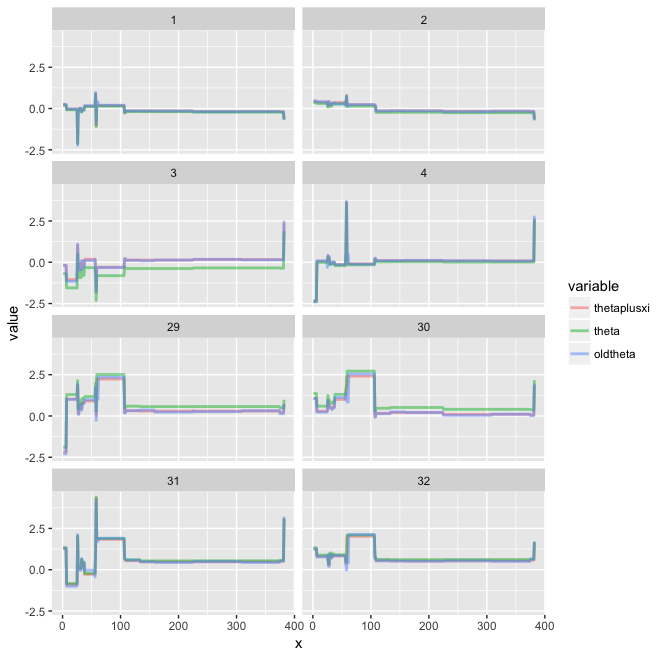
\includegraphics[width=0.9\textwidth]{thetaonly.png}
\caption{ Again, they're very similar to one another except some samples including 3 and 30. And unfortunately, $\Theta + \xi$ is much more well aligned to zero than $\Theta$. The sample-specific effect $\xi$ is not performing as we expected. }
\label{thetaphi}
\end{figure}
















\end{document}






